% Options for packages loaded elsewhere
\PassOptionsToPackage{unicode}{hyperref}
\PassOptionsToPackage{hyphens}{url}
%
\documentclass[
]{article}
\usepackage{lmodern}
\usepackage{amssymb,amsmath}
\usepackage{ifxetex,ifluatex}
\ifnum 0\ifxetex 1\fi\ifluatex 1\fi=0 % if pdftex
  \usepackage[T1]{fontenc}
  \usepackage[utf8]{inputenc}
  \usepackage{textcomp} % provide euro and other symbols
\else % if luatex or xetex
  \usepackage{unicode-math}
  \defaultfontfeatures{Scale=MatchLowercase}
  \defaultfontfeatures[\rmfamily]{Ligatures=TeX,Scale=1}
\fi
% Use upquote if available, for straight quotes in verbatim environments
\IfFileExists{upquote.sty}{\usepackage{upquote}}{}
\IfFileExists{microtype.sty}{% use microtype if available
  \usepackage[]{microtype}
  \UseMicrotypeSet[protrusion]{basicmath} % disable protrusion for tt fonts
}{}
\makeatletter
\@ifundefined{KOMAClassName}{% if non-KOMA class
  \IfFileExists{parskip.sty}{%
    \usepackage{parskip}
  }{% else
    \setlength{\parindent}{0pt}
    \setlength{\parskip}{6pt plus 2pt minus 1pt}}
}{% if KOMA class
  \KOMAoptions{parskip=half}}
\makeatother
\usepackage{xcolor}
\IfFileExists{xurl.sty}{\usepackage{xurl}}{} % add URL line breaks if available
\IfFileExists{bookmark.sty}{\usepackage{bookmark}}{\usepackage{hyperref}}
\hypersetup{
  pdftitle={Assignment3},
  pdfauthor={Stephen Giang},
  hidelinks,
  pdfcreator={LaTeX via pandoc}}
\urlstyle{same} % disable monospaced font for URLs
\usepackage[margin=1in]{geometry}
\usepackage{color}
\usepackage{fancyvrb}
\newcommand{\VerbBar}{|}
\newcommand{\VERB}{\Verb[commandchars=\\\{\}]}
\DefineVerbatimEnvironment{Highlighting}{Verbatim}{commandchars=\\\{\}}
% Add ',fontsize=\small' for more characters per line
\usepackage{framed}
\definecolor{shadecolor}{RGB}{248,248,248}
\newenvironment{Shaded}{\begin{snugshade}}{\end{snugshade}}
\newcommand{\AlertTok}[1]{\textcolor[rgb]{0.94,0.16,0.16}{#1}}
\newcommand{\AnnotationTok}[1]{\textcolor[rgb]{0.56,0.35,0.01}{\textbf{\textit{#1}}}}
\newcommand{\AttributeTok}[1]{\textcolor[rgb]{0.77,0.63,0.00}{#1}}
\newcommand{\BaseNTok}[1]{\textcolor[rgb]{0.00,0.00,0.81}{#1}}
\newcommand{\BuiltInTok}[1]{#1}
\newcommand{\CharTok}[1]{\textcolor[rgb]{0.31,0.60,0.02}{#1}}
\newcommand{\CommentTok}[1]{\textcolor[rgb]{0.56,0.35,0.01}{\textit{#1}}}
\newcommand{\CommentVarTok}[1]{\textcolor[rgb]{0.56,0.35,0.01}{\textbf{\textit{#1}}}}
\newcommand{\ConstantTok}[1]{\textcolor[rgb]{0.00,0.00,0.00}{#1}}
\newcommand{\ControlFlowTok}[1]{\textcolor[rgb]{0.13,0.29,0.53}{\textbf{#1}}}
\newcommand{\DataTypeTok}[1]{\textcolor[rgb]{0.13,0.29,0.53}{#1}}
\newcommand{\DecValTok}[1]{\textcolor[rgb]{0.00,0.00,0.81}{#1}}
\newcommand{\DocumentationTok}[1]{\textcolor[rgb]{0.56,0.35,0.01}{\textbf{\textit{#1}}}}
\newcommand{\ErrorTok}[1]{\textcolor[rgb]{0.64,0.00,0.00}{\textbf{#1}}}
\newcommand{\ExtensionTok}[1]{#1}
\newcommand{\FloatTok}[1]{\textcolor[rgb]{0.00,0.00,0.81}{#1}}
\newcommand{\FunctionTok}[1]{\textcolor[rgb]{0.00,0.00,0.00}{#1}}
\newcommand{\ImportTok}[1]{#1}
\newcommand{\InformationTok}[1]{\textcolor[rgb]{0.56,0.35,0.01}{\textbf{\textit{#1}}}}
\newcommand{\KeywordTok}[1]{\textcolor[rgb]{0.13,0.29,0.53}{\textbf{#1}}}
\newcommand{\NormalTok}[1]{#1}
\newcommand{\OperatorTok}[1]{\textcolor[rgb]{0.81,0.36,0.00}{\textbf{#1}}}
\newcommand{\OtherTok}[1]{\textcolor[rgb]{0.56,0.35,0.01}{#1}}
\newcommand{\PreprocessorTok}[1]{\textcolor[rgb]{0.56,0.35,0.01}{\textit{#1}}}
\newcommand{\RegionMarkerTok}[1]{#1}
\newcommand{\SpecialCharTok}[1]{\textcolor[rgb]{0.00,0.00,0.00}{#1}}
\newcommand{\SpecialStringTok}[1]{\textcolor[rgb]{0.31,0.60,0.02}{#1}}
\newcommand{\StringTok}[1]{\textcolor[rgb]{0.31,0.60,0.02}{#1}}
\newcommand{\VariableTok}[1]{\textcolor[rgb]{0.00,0.00,0.00}{#1}}
\newcommand{\VerbatimStringTok}[1]{\textcolor[rgb]{0.31,0.60,0.02}{#1}}
\newcommand{\WarningTok}[1]{\textcolor[rgb]{0.56,0.35,0.01}{\textbf{\textit{#1}}}}
\usepackage{graphicx,grffile}
\makeatletter
\def\maxwidth{\ifdim\Gin@nat@width>\linewidth\linewidth\else\Gin@nat@width\fi}
\def\maxheight{\ifdim\Gin@nat@height>\textheight\textheight\else\Gin@nat@height\fi}
\makeatother
% Scale images if necessary, so that they will not overflow the page
% margins by default, and it is still possible to overwrite the defaults
% using explicit options in \includegraphics[width, height, ...]{}
\setkeys{Gin}{width=\maxwidth,height=\maxheight,keepaspectratio}
% Set default figure placement to htbp
\makeatletter
\def\fps@figure{htbp}
\makeatother
\setlength{\emergencystretch}{3em} % prevent overfull lines
\providecommand{\tightlist}{%
  \setlength{\itemsep}{0pt}\setlength{\parskip}{0pt}}
\setcounter{secnumdepth}{-\maxdimen} % remove section numbering

\title{Assignment3}
\author{Stephen Giang}
\date{11/20/2020}

\begin{document}
\maketitle

\begin{Shaded}
\begin{Highlighting}[]
\CommentTok{# Problem 1-2}

\KeywordTok{setwd}\NormalTok{(}\StringTok{'C:/Users/Stephen Giang/Documents/Math336Files/data'}\NormalTok{)}
\NormalTok{readData =}\StringTok{ }\KeywordTok{read.csv}\NormalTok{(}\StringTok{'NOAAGlobalT.csv'}\NormalTok{)}

\NormalTok{pacific1 =}\StringTok{ }\KeywordTok{subset}\NormalTok{(readData, LAT }\OperatorTok{>=}\StringTok{ }\DecValTok{-20} \OperatorTok{&}\StringTok{ }\NormalTok{LAT }\OperatorTok{<=}\StringTok{ }\DecValTok{20}\NormalTok{)   }\CommentTok{#20S  - 20N}
\NormalTok{pacific1 =}\StringTok{ }\KeywordTok{subset}\NormalTok{(pacific1, LON }\OperatorTok{>=}\StringTok{ }\DecValTok{160} \OperatorTok{&}\StringTok{ }\NormalTok{LON }\OperatorTok{<=}\StringTok{ }\DecValTok{260}\NormalTok{)  }\CommentTok{#160E - 100W}
\NormalTok{pacific1 =}\StringTok{ }\NormalTok{pacific1[, }\DecValTok{856}\OperatorTok{:}\DecValTok{1455}\NormalTok{]   }\CommentTok{# 01/1951 - 12/2000}

\CommentTok{# -999.9 means missing data so set to 0}
\ControlFlowTok{for}\NormalTok{ ( i }\ControlFlowTok{in} \DecValTok{1}\OperatorTok{:}\KeywordTok{dim}\NormalTok{(pacific1)[}\DecValTok{1}\NormalTok{] ) \{}
  \ControlFlowTok{for}\NormalTok{ ( j }\ControlFlowTok{in} \DecValTok{1}\OperatorTok{:}\KeywordTok{dim}\NormalTok{(pacific1)[}\DecValTok{2}\NormalTok{] ) \{}
    \ControlFlowTok{if}\NormalTok{ (pacific1[i,j] }\OperatorTok{<}\StringTok{ }\DecValTok{-800}\NormalTok{) \{}
\NormalTok{      pacific1[i,j] =}\StringTok{ }\DecValTok{0}
\NormalTok{    \}}
\NormalTok{  \}}
\NormalTok{\}}

\NormalTok{yearDiff =}\StringTok{ }\DecValTok{1999} \OperatorTok{-}\StringTok{ }\DecValTok{1951} \OperatorTok{+}\StringTok{ }\DecValTok{1} 
\NormalTok{pacific =}\StringTok{ }\KeywordTok{matrix}\NormalTok{(}\DecValTok{0}\NormalTok{,}\DataTypeTok{nrow =} \KeywordTok{dim}\NormalTok{(pacific1)[}\DecValTok{1}\NormalTok{], }\DataTypeTok{ncol =}\NormalTok{ yearDiff)}
\CommentTok{# Annual (July - June) Mean Sea Temp}
\ControlFlowTok{for}\NormalTok{ (k }\ControlFlowTok{in} \DecValTok{1}\OperatorTok{:}\NormalTok{yearDiff) \{}
\NormalTok{  pacific[, k] =}\StringTok{ }\KeywordTok{rowMeans}\NormalTok{(pacific1[, (}\DecValTok{12}\OperatorTok{*}\NormalTok{k }\OperatorTok{-}\StringTok{ }\DecValTok{5}\NormalTok{) }\OperatorTok{:}\StringTok{ }\NormalTok{(}\DecValTok{12}\OperatorTok{*}\NormalTok{k }\OperatorTok{+}\StringTok{ }\DecValTok{6}\NormalTok{) ])}
\NormalTok{\}}

\NormalTok{svdPacific =}\StringTok{ }\KeywordTok{svd}\NormalTok{(pacific)}
\NormalTok{D =}\StringTok{ }\KeywordTok{diag}\NormalTok{(svdPacific}\OperatorTok{$}\NormalTok{d)}
\NormalTok{U =}\StringTok{ }\NormalTok{svdPacific}\OperatorTok{$}\NormalTok{u}
\NormalTok{V =}\StringTok{ }\NormalTok{svdPacific}\OperatorTok{$}\NormalTok{v}

\NormalTok{eigVals =}\StringTok{ }\NormalTok{(svdPacific}\OperatorTok{$}\NormalTok{d[}\DecValTok{1}\OperatorTok{:}\DecValTok{10}\NormalTok{])}\OperatorTok{^}\DecValTok{2} \OperatorTok{/}\StringTok{ }\NormalTok{yearDiff}
\NormalTok{eigVals}
\end{Highlighting}
\end{Shaded}

\begin{verbatim}
##  [1] 27.7879120  4.3773517  2.5610076  0.9341387  0.6615021  0.4678065
##  [7]  0.3243314  0.2490007  0.1680932  0.1443271
\end{verbatim}

\begin{Shaded}
\begin{Highlighting}[]
\NormalTok{x =}\StringTok{ }\KeywordTok{seq}\NormalTok{(}\OperatorTok{-}\FloatTok{17.5}\NormalTok{, }\FloatTok{17.5}\NormalTok{, }\DataTypeTok{by=}\DecValTok{5}\NormalTok{)  }\CommentTok{# lat}
\NormalTok{y =}\StringTok{ }\KeywordTok{seq}\NormalTok{(}\FloatTok{162.5}\NormalTok{, }\FloatTok{257.5}\NormalTok{, }\DataTypeTok{by=}\DecValTok{5}\NormalTok{) }\CommentTok{# lon}
\NormalTok{numLatVals =}\StringTok{ }\KeywordTok{length}\NormalTok{(x)}
\NormalTok{numLonVals =}\StringTok{ }\KeywordTok{length}\NormalTok{(y)}
\NormalTok{time =}\StringTok{ }\DecValTok{1951} \OperatorTok{:}\StringTok{ }\DecValTok{1999}

\NormalTok{int=}\KeywordTok{seq}\NormalTok{(}\OperatorTok{-}\FloatTok{0.2}\NormalTok{,}\FloatTok{0.2}\NormalTok{,}\DataTypeTok{length.out=}\DecValTok{81}\NormalTok{)}
\NormalTok{rgb.palette=}\KeywordTok{colorRampPalette}\NormalTok{(}\KeywordTok{c}\NormalTok{(}\StringTok{'black'}\NormalTok{,}\StringTok{'blue'}\NormalTok{, }\StringTok{'darkgreen'}\NormalTok{,}
                               \StringTok{'green'}\NormalTok{, }\StringTok{'yellow'}\NormalTok{,}\StringTok{'pink'}\NormalTok{,}\StringTok{'red'}\NormalTok{,}\StringTok{'maroon'}\NormalTok{),}
                             \DataTypeTok{interpolate=}\StringTok{'spline'}\NormalTok{)}
\KeywordTok{suppressWarnings}\NormalTok{(}\KeywordTok{library}\NormalTok{(maps))}

\NormalTok{umat =}\StringTok{ }\KeywordTok{matrix}\NormalTok{(U[,}\DecValTok{1}\NormalTok{], }\DataTypeTok{nrow =}\NormalTok{ numLonVals)}
\KeywordTok{filled.contour}\NormalTok{(y, x, umat, }\DataTypeTok{color.palette=}\NormalTok{rgb.palette, }\DataTypeTok{levels=}\NormalTok{int,}
               \DataTypeTok{xlim=}\KeywordTok{c}\NormalTok{(}\DecValTok{120}\NormalTok{,}\DecValTok{300}\NormalTok{),}\DataTypeTok{ylim=}\KeywordTok{c}\NormalTok{(}\OperatorTok{-}\DecValTok{40}\NormalTok{,}\DecValTok{40}\NormalTok{),}
               \DataTypeTok{plot.title=}\KeywordTok{title}\NormalTok{(}\DataTypeTok{main=}\StringTok{"EOF1 of the Tropical Pacific Temp Data"}\NormalTok{,}
                                \DataTypeTok{xlab=}\StringTok{"Latitude"}\NormalTok{,}\DataTypeTok{ylab=}\StringTok{"Longitude"}\NormalTok{),}
               \DataTypeTok{plot.axes=}\NormalTok{\{}\KeywordTok{axis}\NormalTok{(}\DecValTok{1}\NormalTok{); }\KeywordTok{axis}\NormalTok{(}\DecValTok{2}\NormalTok{); }\KeywordTok{map}\NormalTok{(}\StringTok{'world2'}\NormalTok{, }\DataTypeTok{add=}\OtherTok{TRUE}\NormalTok{); }\KeywordTok{grid}\NormalTok{()\},}
               \DataTypeTok{key.title=}\KeywordTok{title}\NormalTok{(}\DataTypeTok{main=}\StringTok{"[oC]"}\NormalTok{))}
\end{Highlighting}
\end{Shaded}

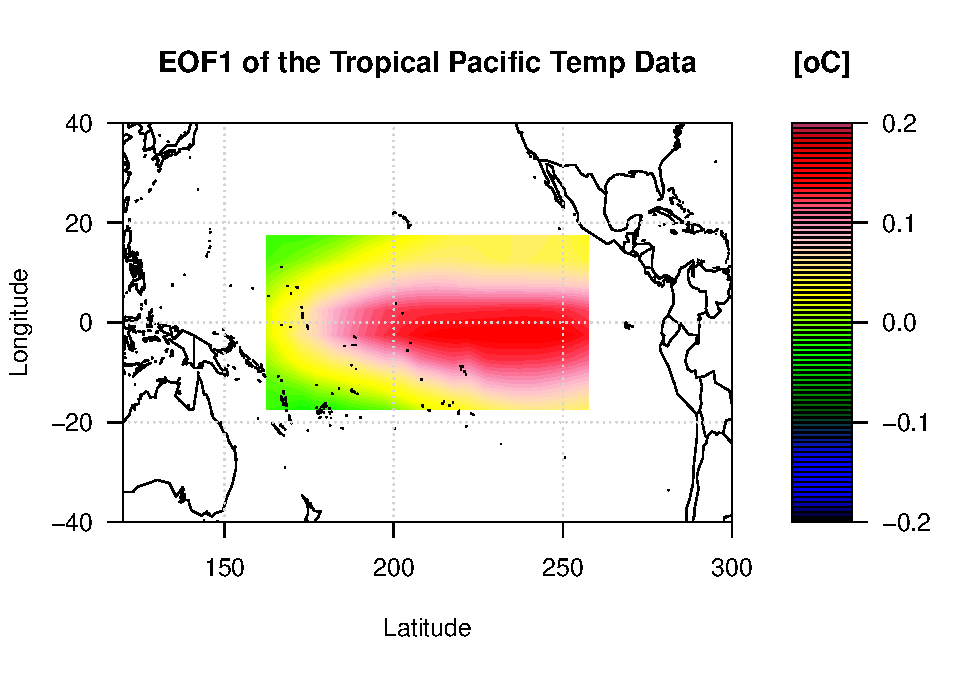
\includegraphics{Assignment3_files/figure-latex/unnamed-chunk-1-1.pdf}

\begin{Shaded}
\begin{Highlighting}[]
\NormalTok{umat =}\StringTok{ }\KeywordTok{matrix}\NormalTok{(U[,}\DecValTok{2}\NormalTok{], }\DataTypeTok{nrow =}\NormalTok{ numLonVals)}
\KeywordTok{filled.contour}\NormalTok{(y, x, umat, }\DataTypeTok{color.palette=}\NormalTok{rgb.palette, }\DataTypeTok{levels=}\NormalTok{int,}
               \DataTypeTok{xlim=}\KeywordTok{c}\NormalTok{(}\DecValTok{120}\NormalTok{,}\DecValTok{300}\NormalTok{),}\DataTypeTok{ylim=}\KeywordTok{c}\NormalTok{(}\OperatorTok{-}\DecValTok{40}\NormalTok{,}\DecValTok{40}\NormalTok{),}
               \DataTypeTok{plot.title=}\KeywordTok{title}\NormalTok{(}\DataTypeTok{main=}\StringTok{"EOF2 of the Tropical Pacific Temp Data"}\NormalTok{,}
                                \DataTypeTok{xlab=}\StringTok{"Latitude"}\NormalTok{,}\DataTypeTok{ylab=}\StringTok{"Longitude"}\NormalTok{),}
               \DataTypeTok{plot.axes=}\NormalTok{\{}\KeywordTok{axis}\NormalTok{(}\DecValTok{1}\NormalTok{); }\KeywordTok{axis}\NormalTok{(}\DecValTok{2}\NormalTok{); }\KeywordTok{map}\NormalTok{(}\StringTok{'world2'}\NormalTok{, }\DataTypeTok{add=}\OtherTok{TRUE}\NormalTok{); }\KeywordTok{grid}\NormalTok{()\},}
               \DataTypeTok{key.title=}\KeywordTok{title}\NormalTok{(}\DataTypeTok{main=}\StringTok{"[oC]"}\NormalTok{))}
\end{Highlighting}
\end{Shaded}

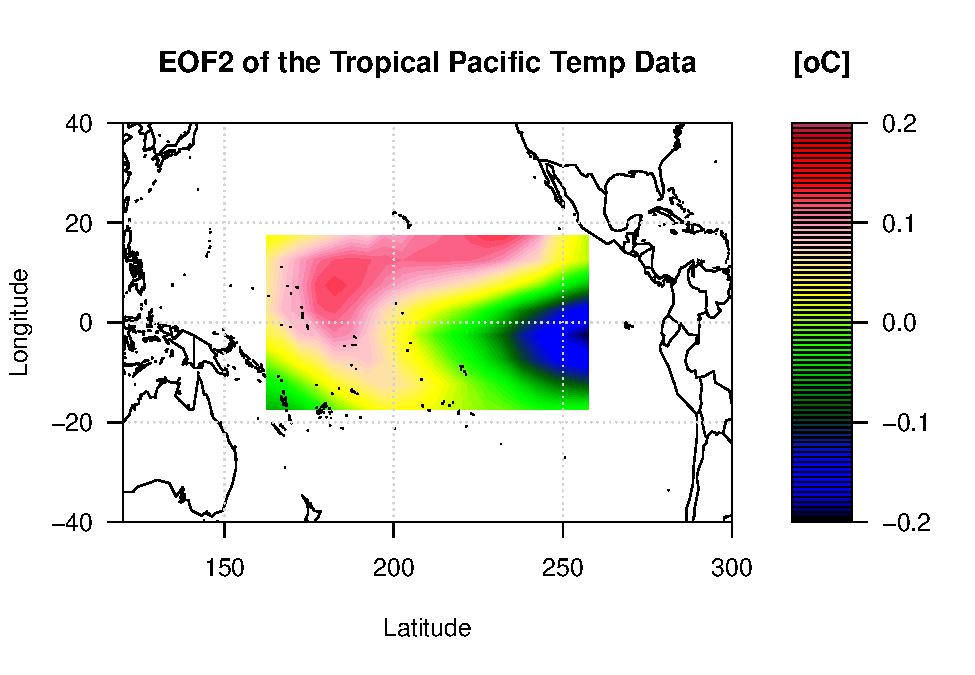
\includegraphics{Assignment3_files/figure-latex/unnamed-chunk-1-2.pdf}

\begin{Shaded}
\begin{Highlighting}[]
\NormalTok{umat =}\StringTok{ }\KeywordTok{matrix}\NormalTok{(U[,}\DecValTok{3}\NormalTok{], }\DataTypeTok{nrow =}\NormalTok{ numLonVals)}
\KeywordTok{filled.contour}\NormalTok{(y, x, umat, }\DataTypeTok{color.palette=}\NormalTok{rgb.palette, }\DataTypeTok{levels=}\NormalTok{int,}
               \DataTypeTok{xlim=}\KeywordTok{c}\NormalTok{(}\DecValTok{120}\NormalTok{,}\DecValTok{300}\NormalTok{),}\DataTypeTok{ylim=}\KeywordTok{c}\NormalTok{(}\OperatorTok{-}\DecValTok{40}\NormalTok{,}\DecValTok{40}\NormalTok{),}
               \DataTypeTok{plot.title=}\KeywordTok{title}\NormalTok{(}\DataTypeTok{main=}\StringTok{"EOF3 of the Tropical Pacific Temp Data"}\NormalTok{,}
                                \DataTypeTok{xlab=}\StringTok{"Latitude"}\NormalTok{,}\DataTypeTok{ylab=}\StringTok{"Longitude"}\NormalTok{),}
               \DataTypeTok{plot.axes=}\NormalTok{\{}\KeywordTok{axis}\NormalTok{(}\DecValTok{1}\NormalTok{); }\KeywordTok{axis}\NormalTok{(}\DecValTok{2}\NormalTok{); }\KeywordTok{map}\NormalTok{(}\StringTok{'world2'}\NormalTok{, }\DataTypeTok{add=}\OtherTok{TRUE}\NormalTok{); }\KeywordTok{grid}\NormalTok{()\},}
               \DataTypeTok{key.title=}\KeywordTok{title}\NormalTok{(}\DataTypeTok{main=}\StringTok{"[oC]"}\NormalTok{))}
\end{Highlighting}
\end{Shaded}

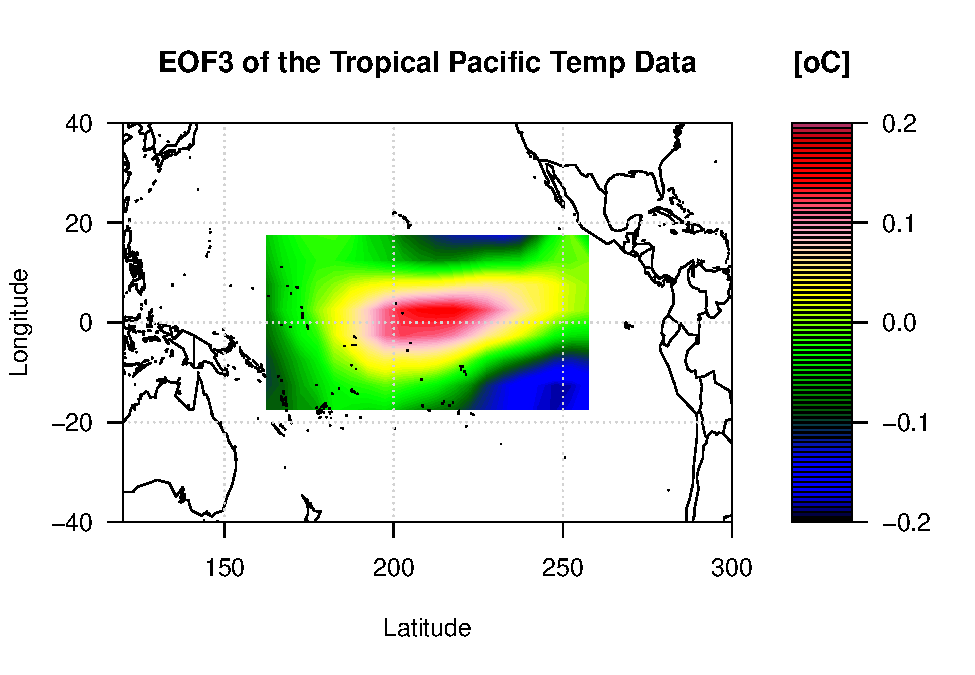
\includegraphics{Assignment3_files/figure-latex/unnamed-chunk-1-3.pdf}

\begin{Shaded}
\begin{Highlighting}[]
\KeywordTok{plot}\NormalTok{(time, V[,}\DecValTok{1}\NormalTok{], }\StringTok{'l'}\NormalTok{, }\DataTypeTok{col =} \StringTok{'black'}\NormalTok{,}
     \DataTypeTok{xlab =} \StringTok{'Year'}\NormalTok{, }\DataTypeTok{ylab =} \StringTok{'PC Scale'}\NormalTok{, }\DataTypeTok{ylim=}\KeywordTok{c}\NormalTok{(}\OperatorTok{-}\FloatTok{0.4}\NormalTok{,}\FloatTok{0.4}\NormalTok{), }
     \DataTypeTok{main =} \StringTok{'The First Three PCs'}\NormalTok{, }\DataTypeTok{panel.first=}\KeywordTok{grid}\NormalTok{())}
\KeywordTok{lines}\NormalTok{(time, V[,}\DecValTok{2}\NormalTok{], }\DataTypeTok{type=}\StringTok{"l"}\NormalTok{, }\DataTypeTok{col=}\StringTok{"blue"}\NormalTok{)}
\KeywordTok{lines}\NormalTok{(time, V[,}\DecValTok{3}\NormalTok{], }\DataTypeTok{type=}\StringTok{"l"}\NormalTok{, }\DataTypeTok{col=}\StringTok{"red"}\NormalTok{)}


\KeywordTok{legend}\NormalTok{(}\DecValTok{1950}\NormalTok{,}\FloatTok{0.4325}\NormalTok{, }\StringTok{'PC1'}\NormalTok{,}\DataTypeTok{lwd=}\DecValTok{2}\NormalTok{ )}
\KeywordTok{legend}\NormalTok{(}\DecValTok{1960}\NormalTok{,}\FloatTok{0.4325}\NormalTok{, }\StringTok{'PC2'}\NormalTok{,}\DataTypeTok{lwd=}\DecValTok{2}\NormalTok{, }\DataTypeTok{col=}\StringTok{"blue"}\NormalTok{)}
\KeywordTok{legend}\NormalTok{(}\DecValTok{1970}\NormalTok{,}\FloatTok{0.4325}\NormalTok{, }\StringTok{'PC3'}\NormalTok{,}\DataTypeTok{lwd=}\DecValTok{2}\NormalTok{, }\DataTypeTok{col=}\StringTok{"red"}\NormalTok{)}
\end{Highlighting}
\end{Shaded}

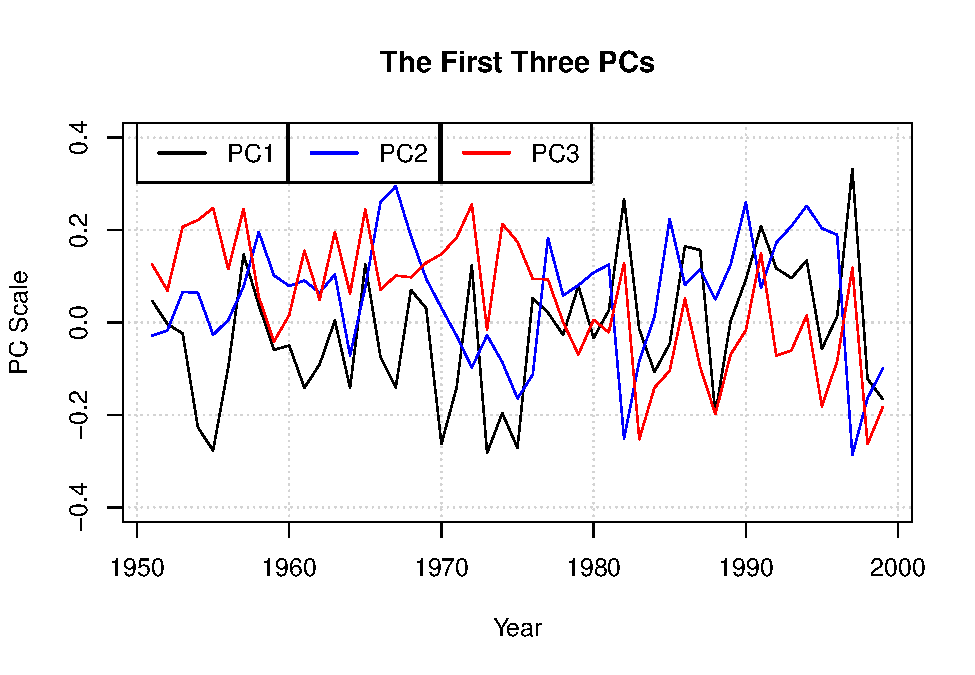
\includegraphics{Assignment3_files/figure-latex/unnamed-chunk-1-4.pdf}

\begin{Shaded}
\begin{Highlighting}[]
\CommentTok{# Problem 3-4}

\KeywordTok{setwd}\NormalTok{(}\StringTok{'C:/Users/Stephen Giang/Documents/Math336Files'}\NormalTok{)}
\NormalTok{readData =}\StringTok{ }\KeywordTok{read.csv}\NormalTok{(}\StringTok{'PrcpRecon5degAnn.csv'}\NormalTok{)}

\NormalTok{pacific =}\StringTok{ }\KeywordTok{subset}\NormalTok{(readData, Lat }\OperatorTok{>=}\StringTok{ }\DecValTok{-20} \OperatorTok{&}\StringTok{ }\NormalTok{Lat }\OperatorTok{<=}\StringTok{ }\DecValTok{20}\NormalTok{)   }\CommentTok{#20S  - 20N}
\NormalTok{pacific =}\StringTok{ }\KeywordTok{subset}\NormalTok{(pacific, Lon }\OperatorTok{>=}\StringTok{ }\DecValTok{160} \OperatorTok{&}\StringTok{ }\NormalTok{Lon }\OperatorTok{<=}\StringTok{ }\DecValTok{260}\NormalTok{)  }\CommentTok{#160E - 100W}
\NormalTok{pacific =}\StringTok{ }\NormalTok{pacific[, }\DecValTok{54}\OperatorTok{:}\DecValTok{102}\NormalTok{] }\CommentTok{#1951 - 1999}

\NormalTok{yearDiff =}\StringTok{ }\DecValTok{1999} \OperatorTok{-}\StringTok{ }\DecValTok{1951} \OperatorTok{+}\StringTok{ }\DecValTok{1}
\NormalTok{svdPacific =}\StringTok{ }\KeywordTok{svd}\NormalTok{(pacific)}
\NormalTok{D =}\StringTok{ }\KeywordTok{diag}\NormalTok{(svdPacific}\OperatorTok{$}\NormalTok{d)}
\NormalTok{U =}\StringTok{ }\NormalTok{svdPacific}\OperatorTok{$}\NormalTok{u}
\NormalTok{V =}\StringTok{ }\NormalTok{svdPacific}\OperatorTok{$}\NormalTok{v}

\NormalTok{eigVals =}\StringTok{ }\NormalTok{(svdPacific}\OperatorTok{$}\NormalTok{d[}\DecValTok{1}\OperatorTok{:}\DecValTok{10}\NormalTok{])}\OperatorTok{^}\DecValTok{2} \OperatorTok{/}\StringTok{ }\NormalTok{yearDiff}
\NormalTok{eigVals}
\end{Highlighting}
\end{Shaded}

\begin{verbatim}
##  [1] 105.4814490  22.2559501   5.4832410   3.3866133   2.8810880   2.1684325
##  [7]   1.4404727   1.2810827   0.9563928   0.7468040
\end{verbatim}

\begin{Shaded}
\begin{Highlighting}[]
\NormalTok{x =}\StringTok{ }\KeywordTok{seq}\NormalTok{(}\OperatorTok{-}\FloatTok{17.5}\NormalTok{, }\FloatTok{17.5}\NormalTok{, }\DataTypeTok{by=}\DecValTok{5}\NormalTok{)  }\CommentTok{# lat}
\NormalTok{y =}\StringTok{ }\KeywordTok{seq}\NormalTok{(}\FloatTok{162.5}\NormalTok{, }\FloatTok{257.5}\NormalTok{, }\DataTypeTok{by=}\DecValTok{5}\NormalTok{) }\CommentTok{# lon}
\NormalTok{numLatVals =}\StringTok{ }\KeywordTok{length}\NormalTok{(x)}
\NormalTok{numLonVals =}\StringTok{ }\KeywordTok{length}\NormalTok{(y)}
\NormalTok{time =}\StringTok{ }\DecValTok{1951} \OperatorTok{:}\StringTok{ }\DecValTok{1999}

\NormalTok{int=}\KeywordTok{seq}\NormalTok{(}\OperatorTok{-}\FloatTok{0.2}\NormalTok{,}\FloatTok{0.2}\NormalTok{,}\DataTypeTok{length.out=}\DecValTok{81}\NormalTok{)}
\NormalTok{rgb.palette=}\KeywordTok{colorRampPalette}\NormalTok{(}\KeywordTok{c}\NormalTok{(}\StringTok{'black'}\NormalTok{,}\StringTok{'blue'}\NormalTok{, }\StringTok{'darkgreen'}\NormalTok{,}
                               \StringTok{'green'}\NormalTok{, }\StringTok{'yellow'}\NormalTok{,}\StringTok{'pink'}\NormalTok{,}\StringTok{'red'}\NormalTok{,}\StringTok{'maroon'}\NormalTok{),}
                             \DataTypeTok{interpolate=}\StringTok{'spline'}\NormalTok{)}
\KeywordTok{suppressWarnings}\NormalTok{(}\KeywordTok{library}\NormalTok{(maps))}

\NormalTok{umat =}\StringTok{ }\KeywordTok{matrix}\NormalTok{(U[,}\DecValTok{1}\NormalTok{], }\DataTypeTok{nrow =}\NormalTok{ numLonVals)}
\KeywordTok{filled.contour}\NormalTok{(y, x, umat, }\DataTypeTok{color.palette=}\NormalTok{rgb.palette, }\DataTypeTok{levels=}\NormalTok{int,}
               \DataTypeTok{xlim=}\KeywordTok{c}\NormalTok{(}\DecValTok{120}\NormalTok{,}\DecValTok{300}\NormalTok{),}\DataTypeTok{ylim=}\KeywordTok{c}\NormalTok{(}\OperatorTok{-}\DecValTok{40}\NormalTok{,}\DecValTok{40}\NormalTok{),}
               \DataTypeTok{plot.title=}\KeywordTok{title}\NormalTok{(}\DataTypeTok{main=}\StringTok{"EOF1 of the Tropical Pacific Precipitation Data"}\NormalTok{,}
                                \DataTypeTok{xlab=}\StringTok{"Latitude"}\NormalTok{,}\DataTypeTok{ylab=}\StringTok{"Longitude"}\NormalTok{),}
               \DataTypeTok{plot.axes=}\NormalTok{\{}\KeywordTok{axis}\NormalTok{(}\DecValTok{1}\NormalTok{); }\KeywordTok{axis}\NormalTok{(}\DecValTok{2}\NormalTok{); }\KeywordTok{map}\NormalTok{(}\StringTok{'world2'}\NormalTok{, }\DataTypeTok{add=}\OtherTok{TRUE}\NormalTok{); }\KeywordTok{grid}\NormalTok{()\},}
               \DataTypeTok{key.title=}\KeywordTok{title}\NormalTok{(}\DataTypeTok{main=}\StringTok{"[oC]"}\NormalTok{))}
\end{Highlighting}
\end{Shaded}

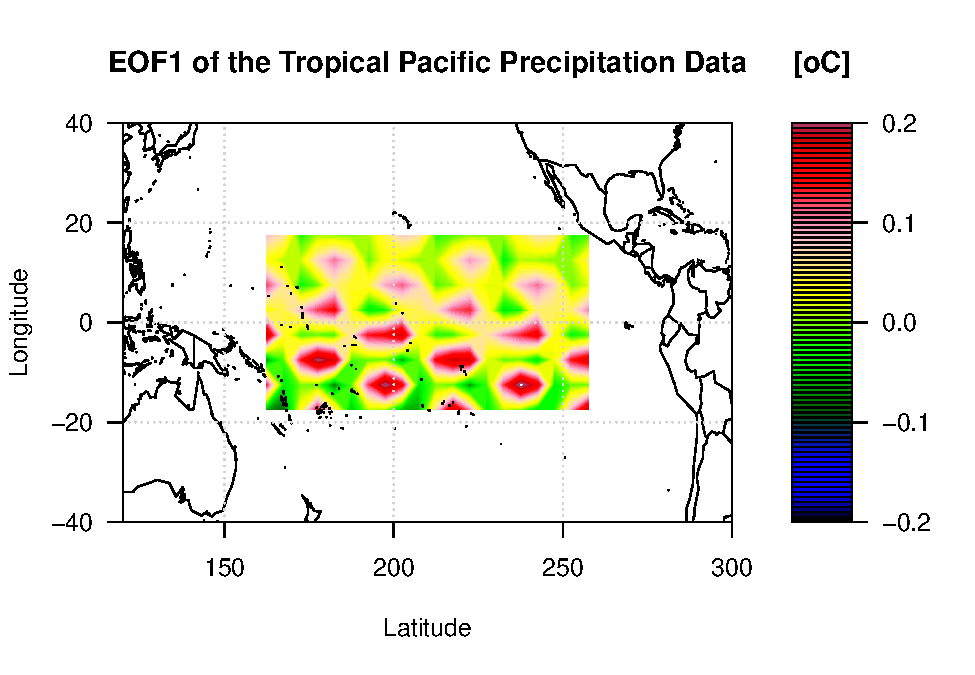
\includegraphics{Assignment3_files/figure-latex/unnamed-chunk-2-1.pdf}

\begin{Shaded}
\begin{Highlighting}[]
\NormalTok{umat =}\StringTok{ }\KeywordTok{matrix}\NormalTok{(U[,}\DecValTok{2}\NormalTok{], }\DataTypeTok{nrow =}\NormalTok{ numLonVals)}
\KeywordTok{filled.contour}\NormalTok{(y, x, umat, }\DataTypeTok{color.palette=}\NormalTok{rgb.palette, }\DataTypeTok{levels=}\NormalTok{int,}
               \DataTypeTok{xlim=}\KeywordTok{c}\NormalTok{(}\DecValTok{120}\NormalTok{,}\DecValTok{300}\NormalTok{),}\DataTypeTok{ylim=}\KeywordTok{c}\NormalTok{(}\OperatorTok{-}\DecValTok{40}\NormalTok{,}\DecValTok{40}\NormalTok{),}
               \DataTypeTok{plot.title=}\KeywordTok{title}\NormalTok{(}\DataTypeTok{main=}\StringTok{"EOF2 of the Tropical Pacific Precipitation Data"}\NormalTok{,}
                                \DataTypeTok{xlab=}\StringTok{"Latitude"}\NormalTok{,}\DataTypeTok{ylab=}\StringTok{"Longitude"}\NormalTok{),}
               \DataTypeTok{plot.axes=}\NormalTok{\{}\KeywordTok{axis}\NormalTok{(}\DecValTok{1}\NormalTok{); }\KeywordTok{axis}\NormalTok{(}\DecValTok{2}\NormalTok{); }\KeywordTok{map}\NormalTok{(}\StringTok{'world2'}\NormalTok{, }\DataTypeTok{add=}\OtherTok{TRUE}\NormalTok{); }\KeywordTok{grid}\NormalTok{()\},}
               \DataTypeTok{key.title=}\KeywordTok{title}\NormalTok{(}\DataTypeTok{main=}\StringTok{"[oC]"}\NormalTok{))}
\end{Highlighting}
\end{Shaded}

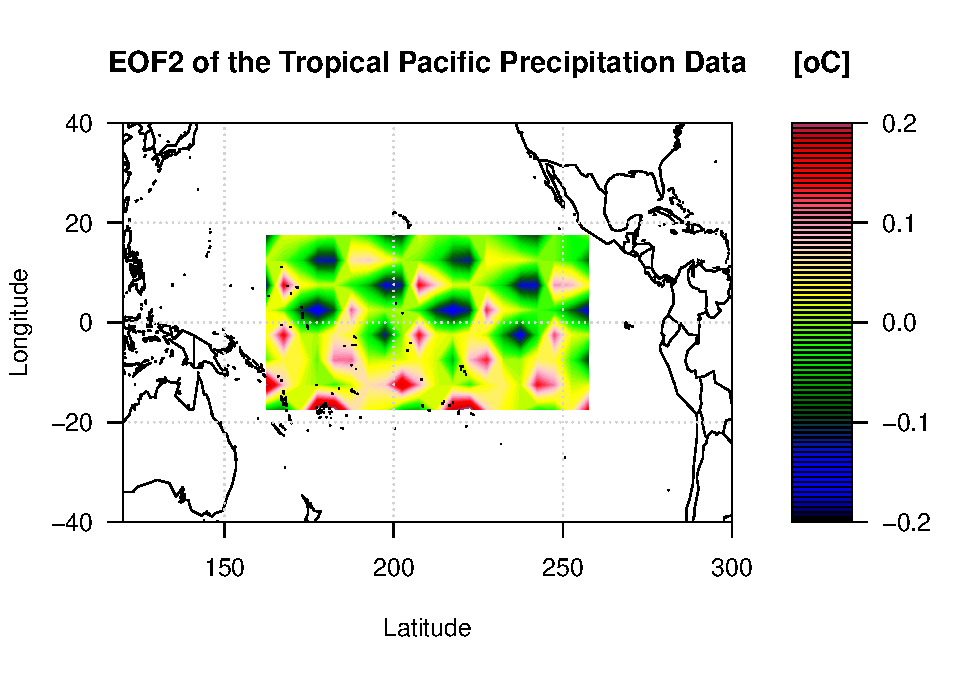
\includegraphics{Assignment3_files/figure-latex/unnamed-chunk-2-2.pdf}

\begin{Shaded}
\begin{Highlighting}[]
\NormalTok{umat =}\StringTok{ }\KeywordTok{matrix}\NormalTok{(U[,}\DecValTok{3}\NormalTok{], }\DataTypeTok{nrow =}\NormalTok{ numLonVals)}
\KeywordTok{filled.contour}\NormalTok{(y, x, umat, }\DataTypeTok{color.palette=}\NormalTok{rgb.palette, }\DataTypeTok{levels=}\NormalTok{int,}
               \DataTypeTok{xlim=}\KeywordTok{c}\NormalTok{(}\DecValTok{120}\NormalTok{,}\DecValTok{300}\NormalTok{),}\DataTypeTok{ylim=}\KeywordTok{c}\NormalTok{(}\OperatorTok{-}\DecValTok{40}\NormalTok{,}\DecValTok{40}\NormalTok{),}
               \DataTypeTok{plot.title=}\KeywordTok{title}\NormalTok{(}\DataTypeTok{main=}\StringTok{"EOF3 of the Tropical Pacific Precipitation Data"}\NormalTok{,}
                                \DataTypeTok{xlab=}\StringTok{"Latitude"}\NormalTok{,}\DataTypeTok{ylab=}\StringTok{"Longitude"}\NormalTok{),}
               \DataTypeTok{plot.axes=}\NormalTok{\{}\KeywordTok{axis}\NormalTok{(}\DecValTok{1}\NormalTok{); }\KeywordTok{axis}\NormalTok{(}\DecValTok{2}\NormalTok{); }\KeywordTok{map}\NormalTok{(}\StringTok{'world2'}\NormalTok{, }\DataTypeTok{add=}\OtherTok{TRUE}\NormalTok{); }\KeywordTok{grid}\NormalTok{()\},}
               \DataTypeTok{key.title=}\KeywordTok{title}\NormalTok{(}\DataTypeTok{main=}\StringTok{"[oC]"}\NormalTok{))}
\end{Highlighting}
\end{Shaded}

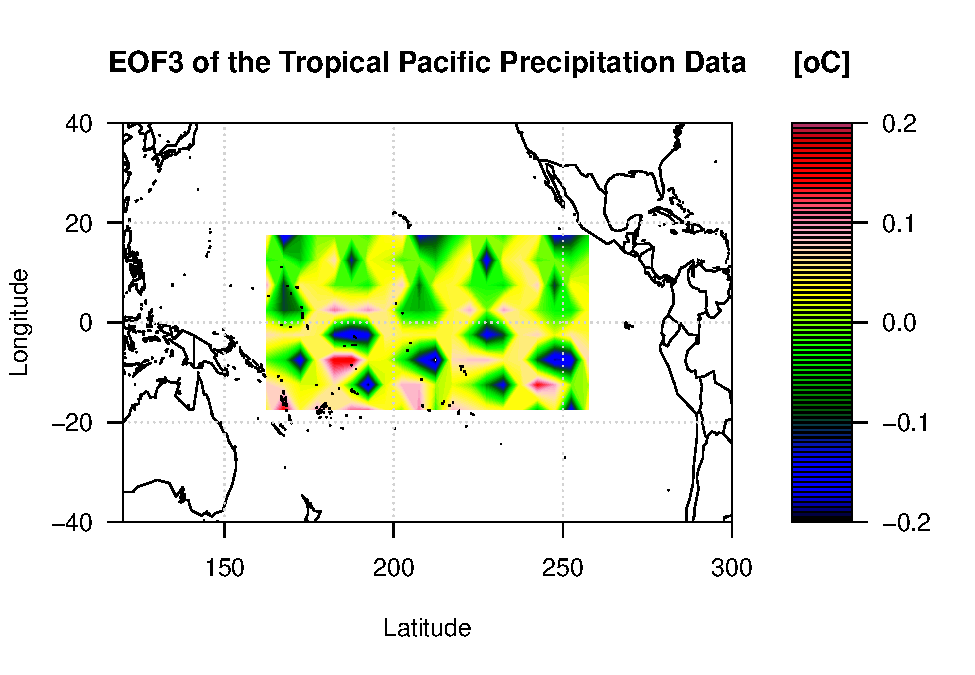
\includegraphics{Assignment3_files/figure-latex/unnamed-chunk-2-3.pdf}

\begin{Shaded}
\begin{Highlighting}[]
\KeywordTok{plot}\NormalTok{(time, V[,}\DecValTok{1}\NormalTok{], }\StringTok{'l'}\NormalTok{, }\DataTypeTok{col =} \StringTok{'black'}\NormalTok{,}
     \DataTypeTok{xlab =} \StringTok{'Year'}\NormalTok{, }\DataTypeTok{ylab =} \StringTok{'PC Scale'}\NormalTok{, }\DataTypeTok{ylim=}\KeywordTok{c}\NormalTok{(}\OperatorTok{-}\FloatTok{0.8}\NormalTok{,}\FloatTok{0.4}\NormalTok{), }
     \DataTypeTok{main =} \StringTok{'The First Three PCs'}\NormalTok{, }\DataTypeTok{panel.first=}\KeywordTok{grid}\NormalTok{())}
\KeywordTok{lines}\NormalTok{(time, V[,}\DecValTok{2}\NormalTok{], }\DataTypeTok{type=}\StringTok{"l"}\NormalTok{, }\DataTypeTok{col=}\StringTok{"blue"}\NormalTok{)}
\KeywordTok{lines}\NormalTok{(time, V[,}\DecValTok{3}\NormalTok{], }\DataTypeTok{type=}\StringTok{"l"}\NormalTok{, }\DataTypeTok{col=}\StringTok{"red"}\NormalTok{)}


\KeywordTok{legend}\NormalTok{(}\DecValTok{1950}\NormalTok{,}\FloatTok{0.448}\NormalTok{, }\StringTok{'PC1'}\NormalTok{,}\DataTypeTok{lwd=}\DecValTok{2}\NormalTok{ )}
\KeywordTok{legend}\NormalTok{(}\DecValTok{1960}\NormalTok{,}\FloatTok{0.448}\NormalTok{, }\StringTok{'PC2'}\NormalTok{,}\DataTypeTok{lwd=}\DecValTok{2}\NormalTok{, }\DataTypeTok{col=}\StringTok{"blue"}\NormalTok{)}
\KeywordTok{legend}\NormalTok{(}\DecValTok{1970}\NormalTok{,}\FloatTok{0.448}\NormalTok{, }\StringTok{'PC3'}\NormalTok{,}\DataTypeTok{lwd=}\DecValTok{2}\NormalTok{, }\DataTypeTok{col=}\StringTok{"red"}\NormalTok{)}
\end{Highlighting}
\end{Shaded}

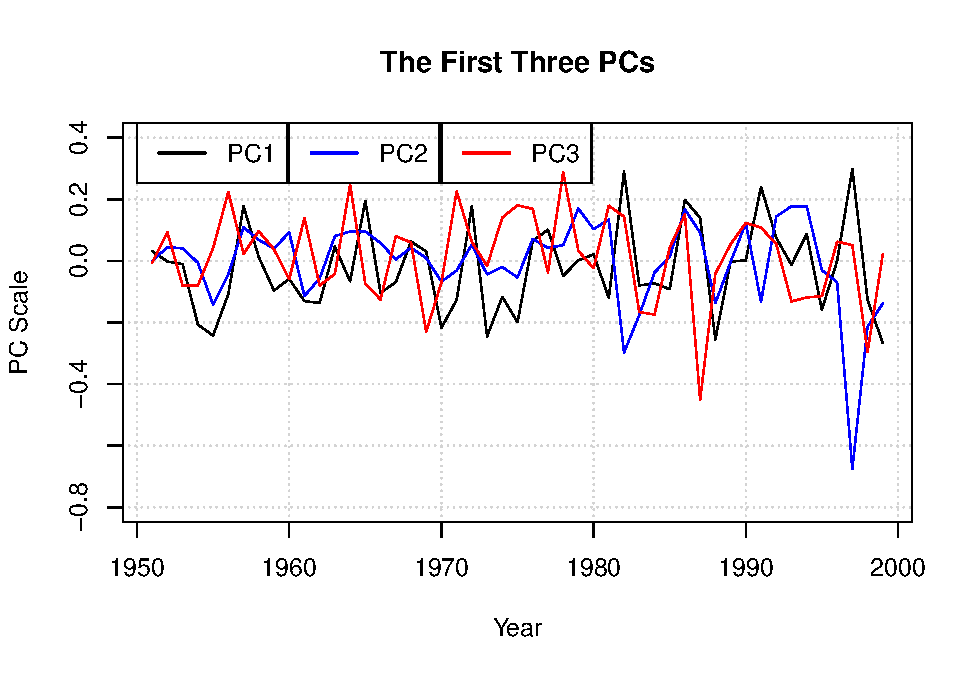
\includegraphics{Assignment3_files/figure-latex/unnamed-chunk-2-4.pdf}

\begin{Shaded}
\begin{Highlighting}[]
\CommentTok{# Problem 8}

\NormalTok{BuffonLongSim =}\StringTok{ }\ControlFlowTok{function}\NormalTok{(d, l, }\DataTypeTok{n =} \DecValTok{10000}\NormalTok{) \{}
\NormalTok{  k =}\StringTok{ }\DecValTok{0}
  \ControlFlowTok{for}\NormalTok{ (i }\ControlFlowTok{in} \DecValTok{1} \OperatorTok{:}\StringTok{ }\NormalTok{n) \{}
\NormalTok{    y =}\StringTok{ }\KeywordTok{runif}\NormalTok{(}\DecValTok{1}\NormalTok{, }\DataTypeTok{min =} \DecValTok{1}\NormalTok{, }\DataTypeTok{max =}\NormalTok{ d)}
\NormalTok{    theta =}\StringTok{ }\KeywordTok{runif}\NormalTok{(}\DecValTok{1}\NormalTok{, }\DataTypeTok{min =} \OperatorTok{-}\NormalTok{pi }\OperatorTok{/}\DecValTok{2}\NormalTok{, }\DataTypeTok{max =}\NormalTok{ pi}\OperatorTok{/}\DecValTok{2}\NormalTok{)}
    \ControlFlowTok{if}\NormalTok{ (y }\OperatorTok{+}\StringTok{ }\NormalTok{l}\OperatorTok{*}\KeywordTok{cos}\NormalTok{(theta) }\OperatorTok{>=}\StringTok{ }\NormalTok{d) \{}
\NormalTok{      k =}\StringTok{ }\NormalTok{k }\OperatorTok{+}\StringTok{ }\DecValTok{1}
\NormalTok{    \}}
\NormalTok{  \}}
  \KeywordTok{return}\NormalTok{(k }\OperatorTok{/}\StringTok{ }\NormalTok{n)}
\NormalTok{\}}

\NormalTok{BuffonLongExact =}\StringTok{ }\ControlFlowTok{function}\NormalTok{(d, l) \{}
\NormalTok{  dl =}\StringTok{ }\NormalTok{d}\OperatorTok{/}\StringTok{ }\NormalTok{l}
\NormalTok{  ld =}\StringTok{ }\NormalTok{l }\OperatorTok{/}\StringTok{ }\NormalTok{d}
\NormalTok{  twopi =}\StringTok{ }\DecValTok{2} \OperatorTok{/}\StringTok{ }\NormalTok{pi}
  \KeywordTok{return}\NormalTok{( twopi }\OperatorTok{*}\StringTok{ }\NormalTok{( }\KeywordTok{acos}\NormalTok{(dl) }\OperatorTok{+}\StringTok{ }\NormalTok{ld }\OperatorTok{-}\StringTok{ }\KeywordTok{sqrt}\NormalTok{( (ld)}\OperatorTok{^}\DecValTok{2} \OperatorTok{-}\StringTok{ }\DecValTok{1}\NormalTok{) ) )}
\NormalTok{\}}


\NormalTok{d =}\StringTok{ }\KeywordTok{floor}\NormalTok{(}\KeywordTok{runif}\NormalTok{(}\DecValTok{1}\NormalTok{, }\DataTypeTok{min =} \DecValTok{1}\NormalTok{, }\DataTypeTok{max =} \DecValTok{100}\NormalTok{))}
\NormalTok{l =}\StringTok{ }\KeywordTok{floor}\NormalTok{(}\KeywordTok{runif}\NormalTok{(}\DecValTok{1}\NormalTok{, }\DataTypeTok{min =} \DecValTok{1}\NormalTok{, }\DataTypeTok{max =} \DecValTok{100}\NormalTok{)) }\OperatorTok{+}\StringTok{ }\NormalTok{d   }\CommentTok{# l > d}

\KeywordTok{BuffonLongSim}\NormalTok{(d, l, }\DecValTok{10000}\NormalTok{)}
\end{Highlighting}
\end{Shaded}

\begin{verbatim}
## [1] 0.9405
\end{verbatim}

\begin{Shaded}
\begin{Highlighting}[]
\KeywordTok{BuffonLongExact}\NormalTok{(d, l)}
\end{Highlighting}
\end{Shaded}

\begin{verbatim}
## [1] 0.9327365
\end{verbatim}

\begin{Shaded}
\begin{Highlighting}[]
\CommentTok{# Problem 9}

\NormalTok{MCSim =}\StringTok{ }\ControlFlowTok{function}\NormalTok{(dim, }\DataTypeTok{n =} \DecValTok{10000}\NormalTok{) \{}
\NormalTok{  x =}\StringTok{ }\KeywordTok{matrix}\NormalTok{(}\KeywordTok{runif}\NormalTok{(dim}\OperatorTok{*}\NormalTok{n, }\DataTypeTok{min=} \DecValTok{-1}\NormalTok{, }\DataTypeTok{max =} \DecValTok{1}\NormalTok{), }\DataTypeTok{ncol =}\NormalTok{ dim)}
\NormalTok{  k =}\StringTok{ }\DecValTok{0}
  \ControlFlowTok{for}\NormalTok{ (i }\ControlFlowTok{in} \DecValTok{1} \OperatorTok{:}\StringTok{ }\NormalTok{n) \{}
    \ControlFlowTok{if}\NormalTok{ ( (}\KeywordTok{t}\NormalTok{(x[i,]) }\OperatorTok\StringTok{ }\NormalTok{x[i,]) }\OperatorTok{<}\StringTok{ }\DecValTok{1}\NormalTok{) \{}
\NormalTok{      k =}\StringTok{ }\NormalTok{k }\OperatorTok{+}\StringTok{ }\DecValTok{1}
\NormalTok{    \}}
\NormalTok{  \}}
  \KeywordTok{return}\NormalTok{( (k}\OperatorTok{/}\NormalTok{n) }\OperatorTok{*}\StringTok{ }\DecValTok{2}\OperatorTok{^}\NormalTok{dim )}
\NormalTok{\}}

\NormalTok{MCExact =}\StringTok{ }\ControlFlowTok{function}\NormalTok{(n,}\DataTypeTok{R=}\DecValTok{1}\NormalTok{) \{}
\NormalTok{  numer =}\StringTok{ }\NormalTok{pi}\OperatorTok{^}\NormalTok{(n}\OperatorTok{/}\DecValTok{2}\NormalTok{)}
\NormalTok{  denom =}\StringTok{ }\KeywordTok{gamma}\NormalTok{((n}\OperatorTok{/}\DecValTok{2}\NormalTok{) }\OperatorTok{+}\StringTok{ }\DecValTok{1}\NormalTok{)}
  \KeywordTok{return}\NormalTok{((numer}\OperatorTok{/}\NormalTok{denom)}\OperatorTok{*}\NormalTok{(R}\OperatorTok{^}\NormalTok{n))}
\NormalTok{\}}


\KeywordTok{MCSim}\NormalTok{(}\DecValTok{8}\NormalTok{, }\DecValTok{100000}\NormalTok{)}
\end{Highlighting}
\end{Shaded}

\begin{verbatim}
## [1] 3.98848
\end{verbatim}

\begin{Shaded}
\begin{Highlighting}[]
\KeywordTok{MCExact}\NormalTok{(}\DecValTok{8}\NormalTok{)}
\end{Highlighting}
\end{Shaded}

\begin{verbatim}
## [1] 4.058712
\end{verbatim}

\begin{Shaded}
\begin{Highlighting}[]
\CommentTok{# Problem 10}


\NormalTok{diceRollSim =}\StringTok{ }\ControlFlowTok{function}\NormalTok{ (n) \{}
\NormalTok{  k =}\StringTok{ }\DecValTok{0}
  \ControlFlowTok{for}\NormalTok{ (i }\ControlFlowTok{in} \DecValTok{1} \OperatorTok{:}\StringTok{ }\NormalTok{n) \{}
\NormalTok{    a =}\StringTok{ }\KeywordTok{floor}\NormalTok{(}\KeywordTok{runif}\NormalTok{(}\DecValTok{1}\NormalTok{, }\DataTypeTok{min =} \DecValTok{1}\NormalTok{, }\DataTypeTok{max =} \DecValTok{6}\NormalTok{))}
\NormalTok{    b =}\StringTok{ }\KeywordTok{floor}\NormalTok{(}\KeywordTok{runif}\NormalTok{(}\DecValTok{1}\NormalTok{, }\DataTypeTok{min =} \DecValTok{1}\NormalTok{, }\DataTypeTok{max =} \DecValTok{6}\NormalTok{))}
    \ControlFlowTok{if}\NormalTok{ (a }\OperatorTok{+}\StringTok{ }\NormalTok{b }\OperatorTok{==}\StringTok{ }\DecValTok{7}\NormalTok{) \{}
\NormalTok{      k =}\StringTok{ }\NormalTok{k }\OperatorTok{+}\StringTok{ }\DecValTok{1}
\NormalTok{    \}}
\NormalTok{  \}}
  \KeywordTok{return}\NormalTok{(k }\OperatorTok{/}\StringTok{ }\NormalTok{n)}
\NormalTok{\}}

\NormalTok{diceRollExact =}\StringTok{ }\ControlFlowTok{function}\NormalTok{ () \{}
\NormalTok{  k =}\StringTok{ }\DecValTok{0}
  \ControlFlowTok{for}\NormalTok{ (i }\ControlFlowTok{in} \DecValTok{1} \OperatorTok{:}\StringTok{ }\DecValTok{6}\NormalTok{) \{}
    \ControlFlowTok{for}\NormalTok{ (j }\ControlFlowTok{in} \DecValTok{1} \OperatorTok{:}\StringTok{ }\DecValTok{6}\NormalTok{) \{}
      \ControlFlowTok{if}\NormalTok{ (i }\OperatorTok{+}\StringTok{ }\NormalTok{j }\OperatorTok{==}\StringTok{ }\DecValTok{7}\NormalTok{) \{}
\NormalTok{        k =}\StringTok{ }\NormalTok{k }\OperatorTok{+}\StringTok{ }\DecValTok{1}
\NormalTok{      \}}
\NormalTok{    \}}
\NormalTok{  \}}
  \KeywordTok{return}\NormalTok{(k }\OperatorTok{/}\StringTok{ }\DecValTok{36}\NormalTok{)}
\NormalTok{\}}

\KeywordTok{diceRollSim}\NormalTok{(}\DecValTok{1000}\NormalTok{)}
\end{Highlighting}
\end{Shaded}

\begin{verbatim}
## [1] 0.155
\end{verbatim}

\begin{Shaded}
\begin{Highlighting}[]
\KeywordTok{diceRollExact}\NormalTok{()}
\end{Highlighting}
\end{Shaded}

\begin{verbatim}
## [1] 0.1666667
\end{verbatim}

\end{document}
